	\documentclass[letterpaper, 11pt]{article}
\usepackage{comment} % enables the use of multi-line comments (\ifx \fi) 
\usepackage{lipsum} %This package just generates Lorem Ipsum filler text. 
\usepackage{fullpage} % changes the margin

\usepackage{fancyhdr} % Required for custom headers
\usepackage{lastpage} % Required to determine the last page for the footer
\usepackage{extramarks} % Required for headers and footers
\usepackage{mdframed}
\usepackage{caption}
\usepackage{subcaption}
\usepackage{float}
\usepackage{array}
\usepackage{soul}
\usepackage{amsmath}
\usepackage{graphicx} % Required to insert images
\usepackage{multicol}
\usepackage{enumitem}
\usepackage{amssymb,bm}
\usepackage{verbatim,eufrak,hyperref,bbm}
\usepackage{titlesec}
\usepackage{listings}

%%%%% TEMPLATE-SPECIFIC FORMATTING %%%%%
%\usepackage{fourier}
\usepackage[adobe-utopia]{mathdesign}
\titleformat{\section}
  {\normalfont\fontsize{12}{15}\bfseries}{\thesection.}{1em}{}
  \titleformat{\subsection}[runin]{\normalfont}{\thesubsection}{3pt}{}
%\usepackage[T1]{fontenc}

%----------------------------------------------------------------------------------------
%	NAME AND CLASS SECTION
%----------------------------------------------------------------------------------------

\newcommand{\hmwkTitle}{Final \ Review\ Solutions} % Assignment title
\newcommand{\hmwkClass}{CME\ 100\ ACE} % Course/class
\newcommand{\hmwkAuthorName}{T Anderson} % Your name
\newcommand{\hmwkAuthorEmail}{timmya@stanford.edu} % Your email

% Set up the header and footer
\pagestyle{fancy}
\lhead{} % Top left header
\chead{} % Top center header
\rhead{} % Top right header
\lfoot{\hmwkClass\ : \hmwkTitle} % Bottom left footer
\cfoot{Page\ \thepage\ of\ \pageref{LastPage}} % Bottom center footer
\rfoot{\hmwkAuthorName} % Bottom right footer
\renewcommand\headrulewidth{0pt} % Size of the header rule
\renewcommand\footrulewidth{0.4pt} % Size of the footer rule


% Math commands
\DeclareMathOperator*{\argmin}{arg\,min}
\DeclareMathOperator*{\argmax}{arg\,max}
\allowdisplaybreaks

% Margins
\topmargin=-0.45in
\evensidemargin=0in
\oddsidemargin=0in
\textwidth=6.5in
\textheight=9.0in
\headsep=0.25in 

\setlength{\parindent}{0pt} % Set indent to zero

\begin{document}

%\thispagestyle{empty}
\noindent
\normalsize 
%\hmwkAuthorName 
\hmwkClass \hfill June\ 10,\ 2017\\
%\hmwkAuthorEmail \\

\begin{center} \Large \textbf{\hmwkTitle} \end{center}

\section{Triple Integrals}
\begin{enumerate}
\item (TC 15.6 \#14) Find the center of mass and moment of inertia about the x-axis of a thin plate bounded by the curves $x = y^2$ and $x = 2y - y^2$ with density $\delta(x,y) = y + 1$.

\par \textbf{Solution:} First we need to calculate the mass:
\[ \int_0^1 \int_{y^2}^{2y - y^2} (y+1) dxdy =2 \int_0^1 (y+1)(y - y^2) dy = \frac{1}{2} \]
From here, calculate the first moments for $x$ and $y$:
\begin{align*}
M_x &= \int_0^1 \int_{y^2}^{2y - y^2} y(y+1) dxdy \\
&= \frac{4}{15} \\
M_y &= \int_0^1 \int_{y^2}^{2y - y^2} x(y+1) dxdy \\
&= \frac{4}{15} \\
\bar x &= \frac{8}{15} \\
\bar y &= \frac{8}{15} \quad\blacksquare 
\end{align*}
For the moment of inertia:
\[ I_x = \int_0^1 \int_{y^2}^{2y - y^2} y^2(y+1) dxdy = \frac{1}{6} \quad\blacksquare \]
Solving problems such as this is mostly a matter of ``plug and chug'', so be sure to have the formulas and their meanings either memorized or on your cheat sheet. 

\item (TC 15.7 \#16) Find the volume of the shape in the following figure. 
\begin{figure}[H]
\centering 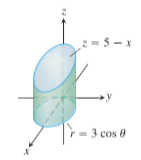
\includegraphics[width=0.15\columnwidth]{finalReviewImgs/TC157_16.png}
\end{figure}

\par \textbf{Solution:} The figure all but gives you that we need to use cylindrical coordinates. The only small catch here is converting the $z$ bounds of integration into cylindrical coordinates, but that is trivially done using $x = r \cos \theta$. So, we set up the integral as:
\begin{align*}
V &= \int_{-\pi/2}^{\pi/2} \int_0^{3 \cos \theta} \int_0^{5 - r \cos \theta} r dz dr d\theta \\
&=  \int_{-\pi/2}^{\pi/2} \int_0^{3 \cos \theta} (5r - r^2 \cos \theta) dr d\theta \\
&= \int_{-\pi/2}^{\pi/2} \left(\frac{45}{2} \cos^2 \theta - 3 \cos^4 \theta\right) d\theta \\
&= \frac{63 \pi}{8} \quad\blacksquare 
\end{align*}


\item (TC 15.7 \#33) Find the volume of the solid between the sphere $\rho = \cos \phi$ and hemisphere $\rho = 2, z \geq 0$. 

\par \textbf{Solution:} Instead of trying to find bounds of integration for the region between the hemisphere and circle, we can simple calculate the volume of each, then subtract the volume of the sphere from the hemisphere.
\[ V_{\text{Hemisphere}} - V_{\text{Sphere}} = \frac{32 \pi}{6} - \frac{\pi}{6} = \frac{31 \pi}{4} \quad\blacksquare \]

\par When you are given problems like this i.e. where you are asked to compute the volume, you should think about what is the actual figure you are being asked to compute, use the fact that volumes are additive, then try to apply known volume formulas. It would have been possible to set up this integral as:
\[ V = \int_0^{2\pi} \int_0^{\pi/2} \int_{\cos \phi}^2 \rho^2 \sin \phi d\rho d \phi d \theta \]
but this is much harder to compute than simple volume formulas. 

\end{enumerate}

\section{Generalized Coordinate Transform}
\begin{enumerate}
\item (TC 15,8 \#2) Find the value of the Jacobian $\partial(x,y)/\partial (u,v)$ for the system:
\begin{gather*}
u = x + 2y \\
v = x - y
\end{gather*}

\par \textbf{Solution:} The most obvious way to solve this problem would be to invert the map $(x,y) \mapsto (u,v)$ to solve for $x$ and $y$ in terms of $(u,v)$. However, this can be a lot of work, and there exists a very easy shortcut. Recall that for an invertible mapping $(x,y) \mapsto (u,v)$, we have
\[ J(x,y) = \frac{1}{J(u,v)} \]
As an aside, this actually is from the much deeper property that the determinant of a matrix inverse is the inverse of the matrix's determinant (say that 5 times fast). 
\par Here, we have a very nice linear mapping between $(x,y)$ and $(u,v)$, so
\[ J(u,v) = \det \left| \begin{array}{cc} 1 & 2 \\ 1 & -1 \end{array} \right| = -3 \]
Therefore, 
\[ J(x,y) = -\frac{1}{3} \quad\blacksquare \]


\item (TC 15.8 \#14) Evaluate the following integral:
\[ \int_0^2 \int_{y/2}^{(y+4)/2} y^3 (2x - y )e^{(2x - y)^2} dx dy \]

\par \textbf{Solution:} In picking the substitutions, note that $2x - y$ shows up in multiple places, so we can pick $u = 2x - y$ and $v = y$. Rearranging this system, we have:
\begin{gather*}
x = \frac{1}{2} (u + v) \\ 
y = v 
\end{gather*}
and then taking the determinant of the matrix for this linear mapping, we have 
\[ \partial(x,y)/\partial(u,v) = \frac{1}{2}\]

\par From here, we need to determine the bounds of integration. Remember the steps for doing this:
\begin{enumerate}[label=\roman*.]
\item Write out the original bounds of integration
\item Substitute in for the new variables
\item Simplify the expressions
\item Sketch the bounds in $(u,v)$ space and find the enclosed region?this will be your region of integration
\end{enumerate}
Following these steps, we can construct the following table:
\begin{center}
\begin{tabular}{ c c c }
 Original Bounds & Substitution & Simplified \\ 
 $y = 0$ & $v = 0$ & $v = 0$ \\  
 $y = 2$ & $v = 2$ & $v = 2$   \\  
 $x = y/2$ & $\frac{1}{2} (u + v) = \frac{1}{2}v$ & $u = 0$   \\  
 $x = (y + 4)/2$ & $\frac{1}{2} (u + v) = (v + 4)/2$ & $ u = 4$
\end{tabular}
\end{center}

So the transformed integral is:
\begin{gather*}
\int_0^2 \int_0^4 \frac{1}{2} v^3 ue^{u^2} dudv  \\
\int_0^2 \frac{1}{4}v^3 \left[ e^{u^2} \right]_0^4 dv \\
(e^{16} - 1) \int_0^2 \frac{1}{4}v^3 dv \\
\frac{1}{16} (e^{16}-1) \left[ v^4 \right]_0^2 \\
e^{16}-1 \quad\blacksquare
\end{gather*}

\end{enumerate}

\section{Line Integrals}
\begin{enumerate}
\item (TC 16.1 \#12) Evaluate $\int_C \sqrt{x^2 + y^2} ds$ along the curve $\bm{r}(t) = 4\cos t \bm{i} + 4 \sin t \bm{j} + 3t \bm{k}$ for $-2\pi \leq t \leq 2\pi$. 

\par \textbf{Solution:} The first step in finding any line integral over a parameterized curve is to calculate the speed:
\[ \frac{ds}{dt} = \left| \frac{d\bm{r}}{dt} \right| = \sqrt{ 16\sin^2 t + 16 \cos^2 t + 9} = 5 \]
Plugging this and the parameterizations into the integral:
\begin{align*}
\int_C \sqrt{x^2 + y^2} ds &= \int_{-2\pi}^{2\pi} \sqrt{ 16\cos^2 t + 16 \sin^2 t} (5)dt \\
&= 20 \int_{-2\pi}^{2\pi} dt\\
&= 80 \pi \quad\blacksquare
\end{align*}


\item (TC 16.1 \#28) Evaluate $f(x,y) = \frac{x + y^2}{\sqrt{1 + x^2}}$ over the curve $C : y = x^2/2$ from $(1,1/2)$ to $(0,0)$. 

\par \textbf{Solution:} We first need to pick a parameterization for the curve. It is usually easiest to pick $x = t$ and $y = f(x(t))$, so we pick
\begin{gather*}
x = t \\
y = \frac{t^2}{2} 
\end{gather*}
and take $1 \geq t \geq 0$. (Normally we would integrate along increasing $t$, but here it is \textit{much} easier to integrate $t$ in the reverse direction.) 

\par From here, calculate the speed:
\[ \frac{ds}{dt} = \sqrt{1 + t^2} \]
Then plugging into the integral:
\begin{align*}
\int_C \frac{x + y^2}{\sqrt{1 + x^2}}ds &= -\int_1^0 \frac{t + \frac{t^4}{4}}{\sqrt{1 + t^2}} \sqrt{1 + t^2} dt \\
&= -\int_1^0 (t + t^4/4) dt \\
&= -\left[ \frac{1}{2} t^2 + \frac{1}{20} t^5 \right]_1^0 \\
&= \frac{11}{20} \quad\blacksquare
\end{align*}

\end{enumerate}

\section{Work}
\begin{enumerate}
\item (TC 16.2 \#20) $\bm{F} = 2y\bm{i} + 3x \bm{j} + (x + y)\bm{k}$ over $\bm{r}(t) = \cos t \bm{i} + \sin t \bm{j} + (t/6)\bm{k}$, $0 \leq t \leq 2 \pi$. 

\par \textbf{Solution:} First find the vector field in terms of the parameterized path:
\[ \bm{F} = 2 \sin t \bm{i} + 3 \cos t \bm{j} + (\sin t + \cos t) \bm{k} \]
then calculate $d \bm{r} / dt$:
\[ \frac{d \bm{r}}{dt} = -\sin t \bm{i} + \cos t \bm{j} + \frac{1}{6} \bm{k} \]
To calculate the integral:
\begin{align*}
\int_0^{2 \pi} \bm{F} \cdot  \frac{d \bm{r}}{dt} dt &= \int_0^{2\pi} \left(3 \cos^2 t - 2 \sin^2 t + \frac{1}{6} \cos t + \frac{1}{6} \sin t\right) dt \\
&= \left[ \frac{3}{2} t + \frac{3}{4} \sin 2t - t + \frac{\sin 2t}{2} + \frac{1}{6} \sin t - \frac{1}{6}\cos t \right]_0^{2\pi} \\
&= \pi \quad\blacksquare
\end{align*}


\item (TC 16.3 \#8) Find the work done by the field $\bm{F} = (y + z)\bm{i} + (x + z) \bm{j} + (x + y) \bm{k}$ when moving on a linear path from $(0,0,0)$ to $(2,4,5)$. 

\par \textbf{Solution:} In general, when you are asked to find the work done when moving between two points but are not given a specific path, you should immediately check if it is a conservative field, and therefore if you can use path independence to calculate the work integral. 
\par It is straightforward to see that the field is conservative. So, we need to solve or the potential function:
\begin{align*}
\frac{\partial \phi}{\partial x} &= y +z \\
\phi &= yx + zx + g(y,z) \\
x + \frac{\partial g}{\partial y} &= x + z \\
g(y,z) &= zy + h(z) \\
x + y + \frac{\partial h}{\partial z} &= x + y \\
h &= C \\
\phi &= yx + xz + zy + C 
\end{align*}
Therefore, we can calculate the work integral as:
\[W = 4(2) + 5(2) + 5(4) = 38 \quad\blacksquare \]


\item (TC 16.3 \#28) Find the potential function for $\bm{F} = e^x \ln y \bm{i} + \left( \frac{ e^x}{y} + \sin z\right) \bm{j} + y\cos z \bm{k}$. 

\par \textbf{Solution:} We follow the same steps to find the potential function as in the previous problem. Namely, we iteratively calculate the potential function by integrating each component of the vector field. (Remember that if a field is conservative, then it is the gradient of some $f(x,y,z)$, and when solving for the potential function we are really just solving for this $f(x,y,z)$.) 
\par Begin with the $\bm{i}$ component, then iteratively solve using the others:
\begin{align*}
\frac{\partial f}{\partial x} &= e^x \ln y \\
f &= e^x \ln y + g(x,y) \\
\frac{e^x}{y} + \frac{\partial g}{\partial y} &= \frac{ e^x}{y} + \sin z \\
g &= y \sin z + h(z)\\
f&= e^x \ln y +  y \sin z + h(z)\\
y \cos z + \frac{\partial h}{\partial z} &= y \cos z \\
h &= C \\
f(x,y,z) &= e^x \ln y +  y \sin z + C \quad\blacksquare
\end{align*}

\end{enumerate}

\section{Flux}
\begin{enumerate}
\item (TC 16.2 \#32) Find the flux of the field $\bm{F} = x^2 \bm{i} + y^2 \bm{j}$ about the closed semicircular path of radius 2 in the upper half plane. 

\par \textbf{Solution:} This of course would be extremely easy to do using Green's theorem, but instead we will do it the long way via line integrals. 
\par The path is split into two parts (the semicircle and the diameter), so it easiest to parameterize the two segments separately then add the flux across each segment together. For the circle we choose $\bm{r} = 2\cos t \bm{i} + 2\sin t \bm{j}$ for $0 \leq t \leq \pi$ and for the diameter we have $\bm{r} = (t - 2) \bm{i}$ for $ 0 \leq t \leq 4$. 

\par Recall the formula for flux:
\[ \text{Flux} = \int_C Mdy - Ndx \]
There are many possible formulas for flux, so the main challenge is choose the most appropriate one. Here, this formula is the most straightforward. We then integrate both segments separately:
\begin{align*}
\text{Flux}_{C_1} &= \int_0^\pi (8\cos^3 t  + 8 \sin^3 t)dt \\
&= \frac{32}{3} \\
\text{Flux}_{C_2} &= \int_0^\pi ((t - 2)^2(0) + 0(1)) dt \\
&= 0 \\
\text{Flux} &= \frac{32}{3} \quad\blacksquare
\end{align*}

%\item (TC 16.2 \#36) Find the flux of $\bm{F} = (x + y) \bm{i} - (x^2 + y^2)\bm{j}$ across the triangle with vertices $(1,0)$, $(0,1)$, and $(-1,0)$.  
%
%\par \textbf{Solution:} Here we need to split the flux calculation up into each of the three edges. We do this because we cannot construct a clean (i.e. differentiable) parameterization that traverses the entire path. Doing this:
%\begin{align*}
%C_1: \bm{r}(t) &= (1-t)\bm{i} + t\bm{j}, \; 0 \leq t \leq 1 \\
%\text{Flux}_1 &= \int 
%\end{align*}


\end{enumerate}

\section{Green's Theorem}
\begin{enumerate}
\item (TC 16.4 \#11) Find the circulation and flux of $\bm{F} = x^3 y^2 \bm{i} + \frac{1}{2} x^4 y \bm{j}$ about the path in the following figure:
\begin{figure}[H]
\centering 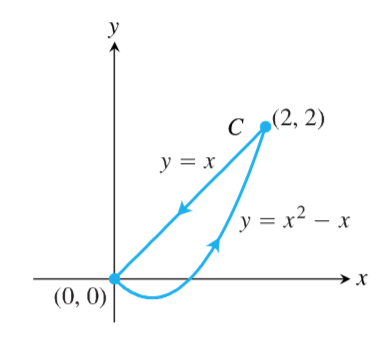
\includegraphics[width=0.2\columnwidth]{finalReviewImgs/TC164_11.png}
\end{figure}
\par \textbf{Solution:} Green's theorem is exceedingly useful since it turns a rather difficult line integral about a closed path into a fairly simple area integral. Recall the work/circulation-curl form of Green's theorem:
\[\oint_{C} (M\, dx + N\, dy) = \iint_{R} \left(\frac{\partial M}{\partial y} - \frac{\partial N}{\partial x}\right)\, dx\, dy \]
So, we simply need to set up the integral on the right and evaluate to find the circulation about the closed path:
\begin{align*}
\text{Circulation} &= \iint_{R} \left(\frac{\partial M}{\partial y} - \frac{\partial N}{\partial x}\right)\, dx\, dy \\
&=  \int_0^2 \int_{x^2 - x}^x \left( 2x^3y - 2 x^3y \right) dy dx \\
&= 0 \quad\blacksquare
\end{align*}

For the flux, recall the flux-divergence form:
\[ \oint_C \bm{F} \cdot d\bm{n} = \iint_R \left( \frac{\partial M}{\partial y} + \frac{\partial N}{\partial x} \right) dxdy \]
so using this we can easily evaluate for the flux: 
\begin{align*}
\text{Flux} &= \iint_R \left( \frac{\partial M}{\partial x} + \frac{\partial N}{\partial y} \right) dxdy \\
&=  \int_0^2 \int_{x^2 - x}^x \left( 3x^2y^2 + \frac{1}{2} x^4 \right) dydx \\
&= \frac{64}{9} \quad\blacksquare
\end{align*}

\par \textit{Note:} Whenever you see flux or circulation about a closed path, you should immediately think to use Green's theorem. 

\item (TC 16.4 \#12) Find the circulation and flux of the field $\bm{F} = \frac{x}{1 + y^2} \bm{i} + \tan^{-1}y \bm{j}$. about the unit circle centered at the origin. 

\par \textbf{Solution:} We follow the exact procedure as above. For the circulation:
\begin{align*}
\text{Circulation} &= \iint_{R} \left( \frac{\partial N}{\partial x} - \frac{\partial M}{\partial y} \right)\, dx\, dy \\
&=  \iint_R  \frac{2yx}{ (1 + y^2)^2 } \, dx\, dy \\
&= \int_{-1}^1 \int_{-\sqrt{1 - y^2}}^{\sqrt{1 -y^2}} \frac{2yx}{ (1 + y^2)^2 } \, dx\, dy \\
&= \int_{-1}^1 0 dy \\
&= 0 \quad\blacksquare
\end{align*}

For the flux:
\begin{align*}
\text{Flux} &= \iint_R \left( \frac{\partial M}{\partial x} + \frac{\partial N}{\partial y} \right)\, dx\, dy \\
&= \int_{-1}^1 \int_{-\sqrt{1 - y^2}}^{\sqrt{1 -y^2}} \left( \frac{1}{1 + y^2} + \frac{1}{1 + y^2} \right) dx dy \\
&= 2 \int_{-1}^1 \int_{-\sqrt{1 - y^2}}^{\sqrt{1 -y^2}} \frac{1}{1 + y^2} dx dy\\
&= 4 \int_{-1}^1\frac{\sqrt{1 - y^2}}{ 1 + y^2} dy 
\end{align*}
This is a rather tricky integral to evaluate. However, we can pick the substitution $ y = \sin(u)$ and the integral becomes somewhat more tractable:
\begin{align*}
4 \int_{-1}^1\frac{\sqrt{1 - y^2}}{ 1 + y^2} dy &= 4 \int_{-\pi/2}^{ \pi/2} \frac{\sqrt{1 - \sin^2(u)}}{ 1 + \sin^2(u)} \cos (u) du \\
&= 4 \int_{-\pi/2}^{ \pi/2} \frac{\cos(u) }{ 1 + \sin^2(u)} \cos (u) du \\
&= 4\int_{-\pi/2}^{ \pi/2} \frac{ \cos^2 (u)}{ 1 + \sin^2 (u)} du \\
&= 4 \int_{-\pi/2}^{\pi/2} \frac{1}{\sec^2(u) +\tan^2(u)} du \\
\intertext{Then, use that $\sec^2(u) -\tan^2(u) = 1$:}
&= 4 \int_{-\pi/2}^{\pi/2} \frac{1}{ 1 + 2 \tan^2(u)} du \\
&= 4 \int_{-\pi/2}^{\pi/2} \frac{1}{ 1 + (\sqrt{2} \tan(u))^2} du  \\
&= 4 \int_{-\pi/2}^{\pi/2} \frac{1+ 1 + 2 \tan^2(u) - (1 + 2 \tan^2(u))}{ 1 + (\sqrt{2} \tan(u))^2} du  \\
&= 4 \int_{-\pi/2}^{\pi/2}\left(  \frac{2 + 2 \tan^2(u)}{ 1 + (\sqrt{2} \tan(u))^2}  - 1\right) du  \\
&= 4 \int_{-\pi/2}^{\pi/2}\left(  \frac{2 \sec^2(u)}{ 1 + (\sqrt{2} \tan(u))^2}  - 1\right) du  \\
&= 4 \left[ \sqrt{2} \tan^{-1}(\sqrt{2}\tan(u)) - u \right]_{-\pi/2}^{\pi/2} \\
&= 4 \sqrt{2} \pi - 4 \pi \quad\blacksquare
\end{align*}

\end{enumerate}

\section{Surface Integrals}
\begin{enumerate}
\item (TC 16.5 \#38) Find the area of the band cut from the paraboloid $x^2 + y^2 - z = 0$ by the plans $z = 2$ and $z = 6$. 

\par \textbf{Solution:} We will parameterize this surface by $x$ and $y$, so $\bm{p} = \bm{k}$ and $\nabla f = 2x \bm{i} + 2y \bm{j} - \bm{k}$. Therefore:
\[ d \sigma = \frac{ |\sqrt{4x^2 + 4y^2 + 1}|}{ |-1|} dxdy = \sqrt{4(x^2 + y^2) + 1}dx dy \]
The projection of the region of integration in the $(x,y)$ plane is the annulus from $ \sqrt{2} \leq r \leq \sqrt{6}$, so we can evaluate the integral as:
\[ \int_0^{2 \pi} \int_{\sqrt{2}}^{\sqrt{6}} \sqrt{ 4r^2 + 1} r dr d\theta = \frac{49}{3} \pi \quad\blacksquare \]

\item (TC 16.6 \#8) Integrate $H(x,y,z) = yz$ over the part of the sphere $x^2 + y^2 + z^2 = 4$ that lies above the cone $z = \sqrt{x^2 + y^2}$. 

\par \textbf{Solution:} This is actually a relatively involved problem since we are dealing with a surface that we do not parameterize by $(x,y)$ or some other combination of variables in our domain. Instead, since we are integrating over a spherical domain, we parameterize the surface by $(\theta,\phi)$. Therefore, the surface is:
\[ S: \bm{r}(\theta,\phi) = 2 \sin \phi\cos \theta \bm{i} + 2 \sin \phi \sin \theta \bm{j} + 2 \cos \phi \bm{k} \]

To figure out the bounds on $\theta$ and $\phi$, note that we have radial symmetry in the $(x,y)$ plane, so $0 \leq \theta \leq 2\pi$. For $\phi$, note that the cone and sphere intersect at $z = 2$, so the upper bound on $\phi$ is $z = 2 = 2 \cos \phi \implies \phi = \frac{\pi}{4}$ and therefore $0 \leq \phi \leq \frac{\pi}{4}$.
\par To compute $d \sigma$, we need to compute $|\bm{r}_\phi \times \bm{r}_\theta|$:
\[ \bm{r}_\phi \times \bm{r}_\theta =\left| \begin{array}{ccc} \bm{i} & \bm{j} & \bm{k}\\ 2 \cos \phi \sin \theta & 2 \sin \phi \sin \theta & - 2 \sin \phi	 \\ -2 \sin \phi \sin \theta & 2 \sin \phi \sin \theta & 0 \end{array} \right| = 4\sin^2 \phi \cos \theta \bm{i} + 4 \sin^2 \phi \sin \theta \bm{j} + 4 \sin \phi \cos \phi \bm{k}  \]
and therefore:
\[ | \bm{r}_\phi \times \bm{r}_\theta| = \sqrt{ 16 \sin^4 \phi \cos^2 \theta + 16 \sin^4 \phi \sin^2 \theta  + 16 \sin^2 \phi \cos^2 \phi } = 4 \sin \phi \]

We can also rewrite $H(\cdot)$ as $H(\theta,\phi) = 4\sin \phi \cos \phi \sin \theta$.
\par Finally, combining these we can write and compute the surface integral:
\begin{align*}
\int_0^{2 \pi} \int_0^{\pi/4} 4\sin \phi \cos \phi \sin \theta (4 \sin \phi)d \phi d \theta &= 16 \int_0^{2 \pi} \int_0^{\pi/4} \sin^2 \phi \cos \phi \sin \theta d \phi d \theta \\
&= 16  \int_0^{\pi/4} \sin^2 \phi \cos \phi \int_0^{2 \pi} \sin \theta d \theta d \phi  \\
&= 0 \quad\blacksquare
\end{align*}

%\item (TC 16.6 \#42) Find the area of the cap cut from the sphere $x^2 + y^2 + z^2 = 2$ by the cone $z = \sqrt{x^2 + y^2}$. 


\end{enumerate}

\section{Flux in 3D}
\begin{enumerate}
\item (TC 16.6 \# 22) Find the outward flux of $\bm{F} = x \bm{i} + y \bm{j} + z \bm{k}$ across the sphere of radius 1. 

\par \textbf{Solution:} We are dealing with a spherical surface, so it is not easily parameterized by any sort of projection into the $(x,y)$ plane. Therefore, we need to use our formulas for computing flux over a parameterized surface. To do this, we first need to choose our parameterization. The surface in question is a sphere, so spherical coordinates are very natural. Therefore, our surface is parameterized as:

\[ S : \bm{r}(\phi,\theta) = \sin \phi\cos \theta \bm{i} + \sin \phi \sin \theta \bm{j} + \cos \phi \bm{k} \]

Recall that for flux, we have the formula:

\[ \text{Flux} = \iint_S \bm{F} \cdot \bm{r}_u \times \bm{r}_v du dv \]

Therefore, we can write this flux integral as:

\[ \text{Flux} = \iint_S \bm{F} \cdot \bm{r}_\phi \times \bm{r}_\theta d\phi d \theta \]

From the previous problem, we know that:
\[ \bm{r}_\phi \times \bm{r}_\theta =\left| \begin{array}{ccc} \bm{i} & \bm{j} & \bm{k}\\  \cos \phi \sin \theta &  \sin \phi \sin \theta & -  \sin \phi	 \\ - \sin \phi \sin \theta &  \sin \phi \sin \theta & 0 \end{array} \right| = \sin^2 \phi \cos \theta \bm{i} + \sin^2 \phi \sin \theta \bm{j} + \sin \phi \cos \phi \bm{k}  \]

To find the bounds on $\phi$ and $\theta$, note that we are integrating over the entire sphere, so $0 \leq \phi \leq \pi$ and $0 \leq \theta \leq 2 \pi$. With this we can finally setup and compute the integral:
\begin{align*}
\iint_S \bm{F} \cdot \bm{r}_\phi \times \bm{r}_\theta d\phi d\theta &= \int_0^{2\pi} \int_0^\pi \sin \phi d\phi d\theta \\
&= 4 \pi \quad\blacksquare
\end{align*}


\end{enumerate}

\section{Stokes' Theorem}
\begin{enumerate}
\item (TC 16.7 \#2) Find the circulation of $\bm{F} = 2y \bm{i} + 3x \bm{j} - z^2 \bm{k}$ about the circle of radius 3 in the $(x,y)$ plane centered at the origin in the counterclockwise direction. 

\par \textbf{Solution:} To apply Stokes' Theorem, we first need to compute the curl:
\[ \nabla \times \bm{F} = \left| \begin{array}{ccc} \partial / \partial x & \partial / \partial y & \partial / \partial z \\  2y &  3x  & -z^2 \end{array} \right| = \bm{k} \]
From here, we need to decide what surface we would like to apply Stokes' Theorem to. Remember that Stokes' Theorem states that the circulation about the edge of a surface is equal to the flux of the curl across the surface. (This is a generalization of the circulation/curl form of Green's theorem to higher dimensions.) Choosing the surface is critical to evaluating a circulation integral using Stokes' Theorem, so you want to choose the simplest surface possible. 

\par Here, we will simply choose the circle of radius 3 in the $(x,y)$ plane centered at the origin. Therefore, the normal vector to our surface is $\bm{n} = \bm{k}$. 

\par Now, recall the definition of Stokes' Theorem:
\[ \oint_C \bm{F} \cdot d \bm{r} = \iint_S \nabla \times \bm{F} \cdot \bm{n} d \sigma \]
We have calculated the curl and the normal vector, so all that is left is $d \sigma$. However, we are integrating a flat surface in the $(x,y)$ plane, so $d \sigma = dx dy$. Finally, we can write the integral as:
\begin{align*}
\oint_C \bm{F} \cdot d \bm{r} &= \iint_S \nabla \times \bm{F} \cdot \bm{n} d \sigma \\
&= \iint_S \bm{k} \cdot \bm{k} dx dy \\
&= \iint_S dx dy \\
&= 9 \pi \quad\blacksquare
\end{align*}


\item (TC 16.7 \#18) Find the flux of the curl of $\bm{F} = y^2 \bm{i} + z^2 \bm{j} + x \bm{k}$ across the surface $\bm{r}(\phi,\theta) = 2 \sin \phi \cos \theta \bm{i} + 2 \sin \phi\sin \theta\bm{j} + 2\cos \phi \bm{k}$, $ 0 \leq \phi \leq \pi/2$, $0 \leq \theta \leq 2 \pi$. 

\par \textbf{Solution:} We first need to calculate the curl:
\[ \nabla \times \bm{F} = \left| \begin{array}{ccc} \partial / \partial x & \partial / \partial y & \partial / \partial z \\  y^2 &  z^2  & x \end{array} \right| = - 2z \bm{i} - \bm{j} - 2y \bm{k}  \]
Remember that we can rewrite the flux of the curl integral as:
\[ \iint_S \nabla \times \bm{F} \cdot \bm{n} d\sigma = \iint_S \nabla \times \bm{F} \cdot \bm{r}_u \times \bm{r}_v dudv \]
Since we are dealing with a parameterized surface, this is the form we will use. 
\par Note that we are just integrating over the surface of a hemisphere of radius 2. so from above, we have:
\[ \bm{r}_\phi \times \bm{r}_\theta =\left| \begin{array}{ccc} \bm{i} & \bm{j} & \bm{k}\\ 2 \cos \phi \sin \theta & 2 \sin \phi \sin \theta & - 2 \sin \phi	 \\ -2 \sin \phi \sin \theta & 2 \sin \phi \sin \theta & 0 \end{array} \right| = 4\sin^2 \phi \cos \theta \bm{i} + 4 \sin^2 \phi \sin \theta \bm{j} + 4 \sin \phi \cos \phi \bm{k}  \]
The bounds of integration are given in the problem, so we can finally assemble the integral and solve:
\begin{align*}
\nabla \times \bm{F}  &= - 2z \bm{i} - \bm{j} - 2y \bm{k} \\
&= -4 \cos \phi \bm{i} - \bm{j} - 4\sin \phi \sin\theta \bm{k} \\
 \iint_S \nabla \times \bm{F} \cdot \bm{n} d\sigma &= \int_0^{2\pi} \int_0^{\pi/2} \nabla \times \bm{F} \cdot \bm{r}_\phi \times \bm{r}_\theta d\phi d\theta \\
 &= \int_0^{2\pi} \int_0^{\pi/2} (-16 \sin^2 \phi \cos \phi \cos \theta - 4 \sin^2 \phi \sin \theta - 16 \sin^2 \phi \sin \theta \cos \theta)d \phi d \theta \\
 &= \int_0^{\pi/2} \int_0^{2\pi} (-16 \sin^2 \phi \cos \phi \cos \theta - 4 \sin^2 \phi \sin \theta - 16 \sin^2 \phi \sin \theta \cos \theta) d \theta d \phi 
\end{align*}
Note that each term in this integral contains a single trigonometric function in $\theta$, so evaluating the integral over $0 \leq \theta\leq 2 \pi$ is identically zero for each term. Therefore, we have:
\[ \int_0^{2\pi} \int_0^{\pi/2} \nabla \times \bm{F} \cdot \bm{r}_\phi \times \bm{r}_\theta d\phi d\theta = 0 \quad\blacksquare \]
\end{enumerate}

\section{Divergence Theorem}
\begin{enumerate}
\item (TC 16.8 \#6) Find the outward flux of $\bm{F} = x^2 \bm{i} + y^2 \bm{j} + z^2 \bm{k}$ across the boundary of the unit cube in the first octant. 

\par \textbf{Solution:} Solving problems using the divergence theorem is very straight forward: calculate the divergence, then integrate the divergence over the volume. 
\par We first find the divergence:
\[ \nabla \cdot \bm{F} = 2x + 2y + 2z \]
Then integrate this over the region:
\begin{align*}
\text{Flux} &= \int_0^1 \int_0^1 \int_0^1 (2x + 2y + 2z) dxdydz \\
&= 3 \quad\blacksquare 
\end{align*}


\textit{Note:} you should almost always go to the divergence theorem when you are asked to find the flux over a closed surface. Furthermore, it is very easy to determine if the divergence is zero. If it is, you automatically know the net flux will be zero and you are done. 

\item (TC 16.8 \#15) Find the flux of $\bm{F} = (5x^3 + 12xy^2)\bm{i} + (y^3+ e^y\sin z)\bm{j} + (5z^3 + e^y \cos z)\bm{k}$ across the boundary of the volume between the spheres $x^2 + y^2 + z^2 =1 $ and $x^2 + y^2 + z^2 = 2$.

\par \textbf{Solution:} Once again, find the divergence, then integrate over the volume:
\[ \nabla \cdot \bm{F} = 15 x^2 + 12 y^2 + 3y^2 + e^y\sin z + 15z^2  - e^y \sin z = 15x^2 + 15y^2 + 15z^2 \]
From here, recall that using the divergence theorem is just computing a volume integral, and volume integrals are additive. Therefore, to compute the flux, we can simply integrate the divergence over both spheres, then subtract the flux of the inner sphere's boundary from the outer spheres:
\begin{align*} 
\text{Flux}_{\text{Outer}} &= \int_0^{2 \pi} \int_0^\pi \int_0^{\sqrt{2}} 15 \rho^2 (\rho^2 \sin \phi) d\rho d\phi d\theta \\
&= 12 \sqrt{2} \int_0^{2\pi} \int_0^\pi \sin \phi d\phi d\theta \\
&= 48 \sqrt{2} \pi \\
\text{Flux}_{\text{Inner}} &=  \int_0^{2 \pi} \int_0^\pi \int_0^{1} 15 \rho^2 (\rho^2 \sin \phi) d\rho d\phi d\theta \\
&= 3 \int_0^{2\pi} \int_0^\pi \sin \phi d\phi d\theta \\
&= 6 \int_0^{2\pi} d\theta \\
&= 12 \pi \\
\text{Flux}_{\text{Outer}} - \text{Flux}_{\text{Inner}} &= (48\sqrt{2} - 12) \pi \quad\blacksquare
\end{align*}

\end{enumerate}



\end{document}